\tikzstyle{vertex} = [circle, minimum size=10pt, text=black, very thick, draw=black!55, top color=white,bottom color=black!20]

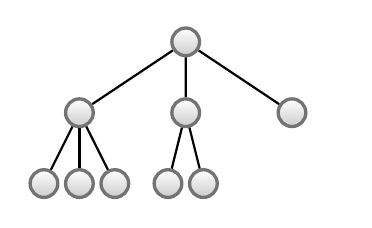
\begin{tikzpicture}[scale=0.9,level distance=1cm,level 1/.style={sibling distance=1.5cm}, level 2/.style={sibling distance=.5cm},edge from parent/.style={draw,thick}]
  \useasboundingbox (-2.23,-2.23) rectangle (2.23,0.2);
  \node[vertex] {}
    child {node[vertex] {}
      child {node[vertex] {}}
      child {node[vertex] {}}
      child {node[vertex] {}}
    }
    child {node[vertex] {}
      child {node[vertex] {}}
      child {node[vertex] {}}
    }
    child {node[vertex] {}
    }
  ;


\end{tikzpicture}

